\documentclass{article}
\usepackage[utf8]{inputenc}

% Page setup
\usepackage[a4paper,landscape,margin=2cm]{geometry}
\usepackage{amsmath}

% Typography
\usepackage[scaled]{helvet}
\let\familydefault\sfdefault

\usepackage[usenames,svgnames]{xcolor}
\usepackage{tikz,pgfplots}
\usetikzlibrary{positioning,arrows,intersections}

\definecolor{colordelta}    {RGB}{199,212,104}
\definecolor{colorsnapshot} {RGB}{79 ,142,209}
\definecolor{colordict}     {RGB}{143,232,186}
\definecolor{colorhdt}      {RGB}{49 ,167,226}
\definecolor{colortext}     {RGB}{29 ,29 ,27 }

\begin{document}
\pagestyle{empty}
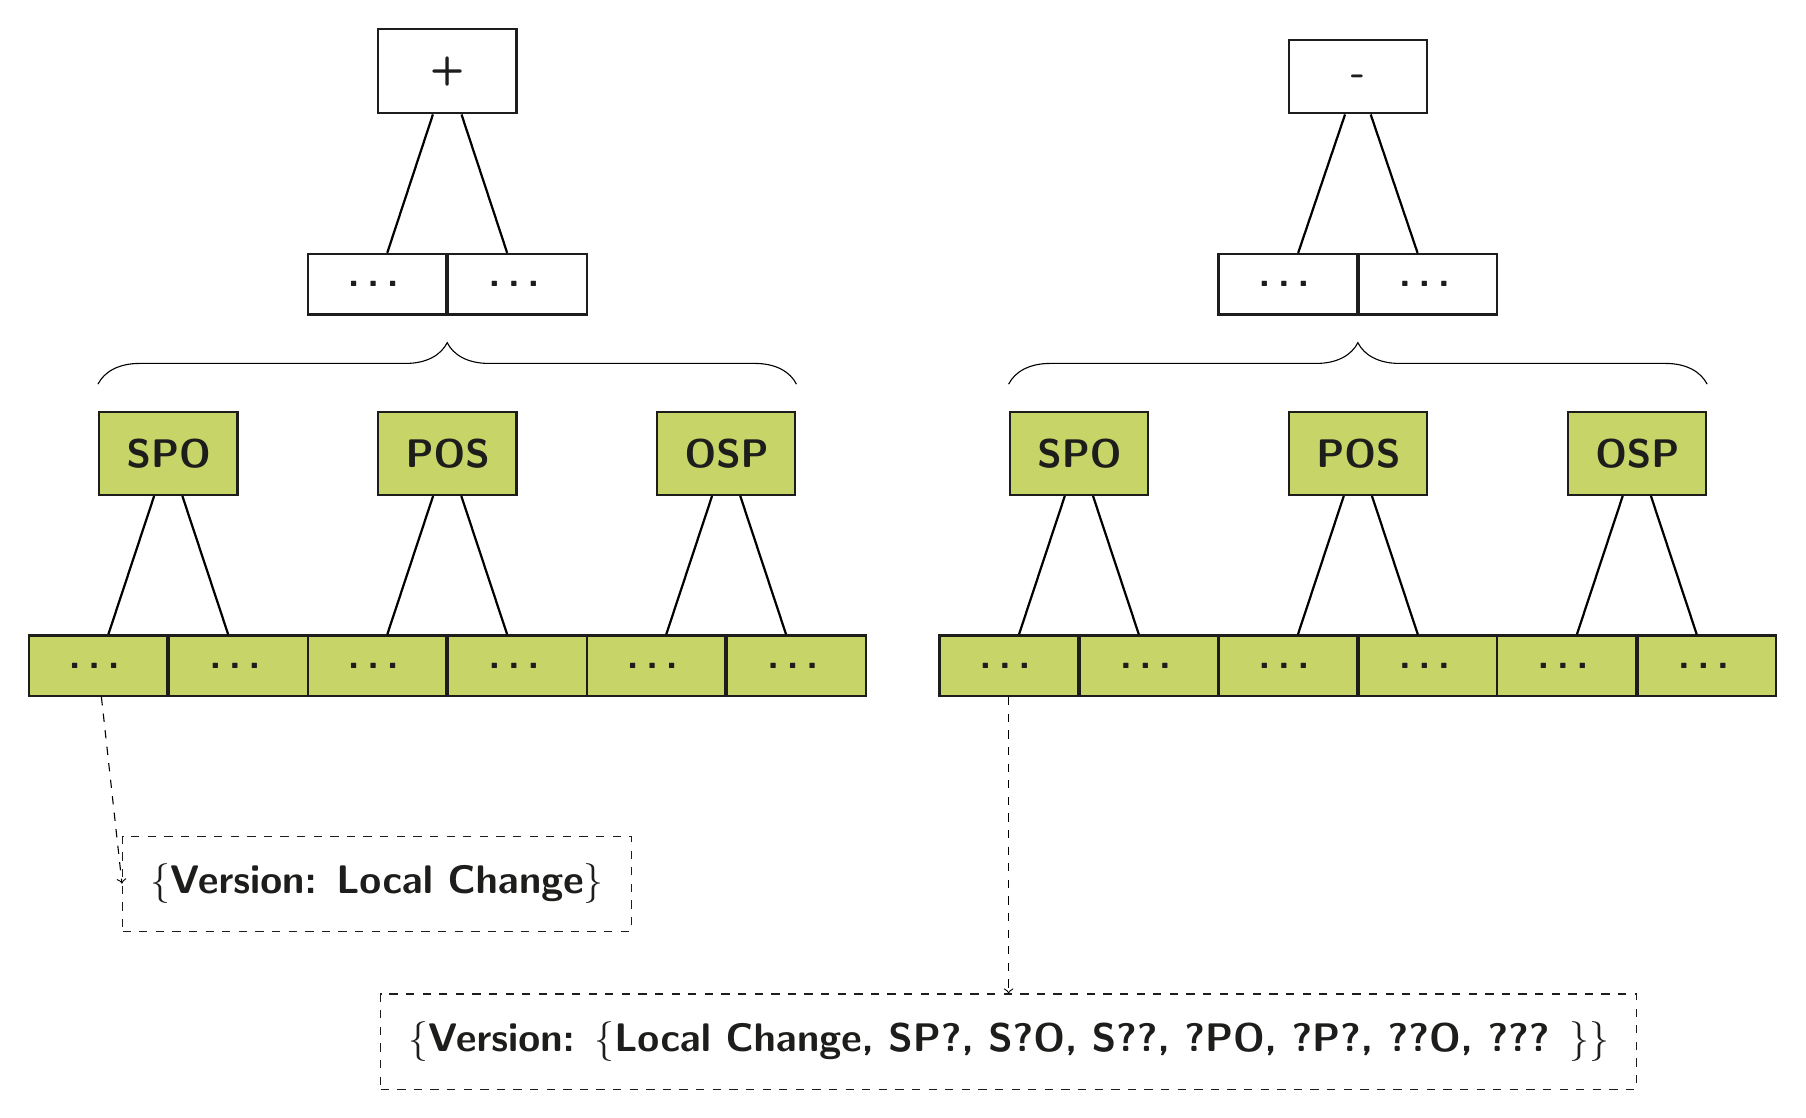
\begin{tikzpicture}[
    node distance = 5em, auto,
    font={\Large\itshape},
    base/.style={text=colortext,font={\Large\bfseries},inner sep=10pt,align=center,rectangle},
    txt/.style={text=colortext,font={\Large\bfseries},align=center},
    treenode/.style={base,thick,draw=colortext,text width=3em},
    relation/.style={text width=13em},
]
    
    % Text
    %\node[txt,below=of delta5]             {5};
    
    % Arrows
    %\draw[->,thick](delta1) to [out=135,in=45] (snapshot);
    
    % Brace around snapshot and delta's
    %\draw [decorate, decoration={brace,mirror,amplitude=15pt,raise=55pt}] (snapshot.west) -- (snapshot.east);
    %\draw [decorate, decoration={brace,mirror,amplitude=15pt,raise=55pt}] (delta1.west) -- (delta5.east);
    
    % Additions trees    
    \node[treenode,fill=colordelta] (asporoot)        {SPO};
    \node[treenode,fill=colordelta,below=of asporoot.south west] (aspo1) {\ldots};
    \node[treenode,fill=colordelta,below=of asporoot.south east] (aspo2) {\ldots};
    \draw[-,thick](aspo1) -- (asporoot);
    \draw[-,thick](aspo2) -- (asporoot);
    \node[treenode,fill=colordelta,right=of asporoot] (aposroot)        {POS};
    \node[treenode,fill=colordelta,below=of aposroot.south west] (apos1) {\ldots};
    \node[treenode,fill=colordelta,below=of aposroot.south east] (apos2) {\ldots};
    \draw[-,thick](apos1) -- (aposroot);
    \draw[-,thick](apos2) -- (aposroot);
    \node[treenode,fill=colordelta,right=of aposroot] (aosproot)        {OSP};
    \node[treenode,fill=colordelta,below=of aosproot.south west] (aosp1) {\ldots};
    \node[treenode,fill=colordelta,below=of aosproot.south east] (aosp2) {\ldots};
    \draw[-,thick](aosp1) -- (aosproot);
    \draw[-,thick](aosp2) -- (aosproot);
    
    % Additions tree
    \node[above=of aposroot]           (adummy) {};
    \node[treenode,above=of adummy] (additionsroot)        {+};
    \node[treenode,below=of additionsroot.south west] (additions1) {\ldots};
    \node[treenode,below=of additionsroot.south east] (additions2) {\ldots};
    \draw[-,thick](additions1) -- (additionsroot);
    \draw[-,thick](additions2) -- (additionsroot);
    \draw [decorate, decoration={brace,amplitude=15pt,raise=25pt}] (asporoot.west) -- (aosproot.east);
    
    \node[base,dashed,draw=colortext,below=of apos1] (aversion) {\{Version: Local Change\}};
    \draw[->,dashed](aspo1) to (aversion.west);
    
    % Dummy nodes for spacing
    \node[right=of asporoot]           (dummy1) {};
    \node[right=of dummy1]             (dummy2) {};
    \node[right=of dummy2]             (dummy3) {};
    \node[right=of dummy3]             (dummy4) {};
    
    % Deletion trees    
    \node[treenode,fill=colordelta,right=of dummy4] (dsporoot)        {SPO};
    \node[treenode,fill=colordelta,below=of dsporoot.south west] (dspo1) {\ldots};
    \node[treenode,fill=colordelta,below=of dsporoot.south east] (dspo2) {\ldots};
    \draw[-,thick](dspo1) -- (dsporoot);
    \draw[-,thick](dspo2) -- (dsporoot);
    \node[treenode,fill=colordelta,right=of dsporoot] (dposroot)        {POS};
    \node[treenode,fill=colordelta,below=of dposroot.south west] (dpos1) {\ldots};
    \node[treenode,fill=colordelta,below=of dposroot.south east] (dpos2) {\ldots};
    \draw[-,thick](dpos1) -- (dposroot);
    \draw[-,thick](dpos2) -- (dposroot);
    \node[treenode,fill=colordelta,right=of dposroot] (dosproot)        {OSP};
    \node[treenode,fill=colordelta,below=of dosproot.south west] (dosp1) {\ldots};
    \node[treenode,fill=colordelta,below=of dosproot.south east] (dosp2) {\ldots};
    \draw[-,thick](dosp1) -- (dosproot);
    \draw[-,thick](dosp2) -- (dosproot);
    
    \node[above=of dposroot]           (ddummy) {};
    \node[treenode,above=of ddummy] (deletionsroot)        {-};
    \node[treenode,below=of deletionsroot.south west] (deletions1) {\ldots};
    \node[treenode,below=of deletionsroot.south east] (deletions2) {\ldots};
    \draw[-,thick](deletions1) -- (deletionsroot);
    \draw[-,thick](deletions2) -- (deletionsroot);
    \draw [decorate, decoration={brace,amplitude=15pt,raise=25pt}] (dsporoot.west) -- (dosproot.east);
    
    \node[below=of dspo1]             (ddummy1) {};
    \node[base,dashed,draw=colortext,below=of ddummy1] (dversion) {\{Version: \{Local Change, SP?, S?O, S??, ?PO, ?P?, ??O, ??? \}\}};
    \draw[->,dashed](dspo1) to (dversion);

\end{tikzpicture}
\end{document}
